% ICSEE 2026 poster — 90 cm × 125 cm (portrait)
\documentclass[
  fontsize=22pt,
  size=custom,
  width=90,
  height=125,
  scale=1.0,
  innermargin=1.4cm,
  outermargin=1.0cm,
  blockverticalspace=0.9cm,
  colspace=1.1cm,
  subcolspace=0.6cm,
]{tikzposter}

% Force exact poster dimensions (90 cm × 125 cm portrait)
\usepackage{geometry}
\geometry{paperwidth=90cm,paperheight=125cm,left=1cm,right=1cm,top=1cm,bottom=1cm}

\usepackage[utf8]{inputenc}
\usepackage[T1]{fontenc}
\usepackage{lmodern}
\usepackage{graphicx}
\usepackage{booktabs}
\usepackage{amsmath}
\usepackage{url}
\usepackage{qrcode}
\usepackage{tikz}
\usetikzlibrary{positioning,arrows.meta,calc}

\definecolor{PosterBlue}{HTML}{0B3D6E}
\definecolor{PosterTeal}{HTML}{0E7490}
\definecolor{PosterLight}{HTML}{E8F4F8}
\definecolor{PosterAccent}{HTML}{F59E0B}
\definecolor{PosterGray}{HTML}{374151}

\definecolorstyle{SimpleStyle}{
  \colorlet{backgroundcolor}{white}
  \colorlet{framecolor}{PosterBlue}
  \colorlet{titlefgcolor}{white}
  \colorlet{titlebgcolor}{PosterBlue}
  \colorlet{blocktitlebgcolor}{PosterTeal}
  \colorlet{blocktitlefgcolor}{white}
  \colorlet{blockbodybgcolor}{PosterLight}
  \colorlet{blockbodyfgcolor}{PosterGray}
}{}
\usecolorstyle{SimpleStyle}
\usebackgroundstyle{Empty}

\title{Integrated Platform for Dynamic GNN ETA Prediction: Dataset Generation \& Testing}

\author{Guy Tordjman \quad\textbar\quad Nadav Voloch}

\institute{The Open University, Ra'anana \textbar{} Ruppin Academic Center, Emek Hefer \textbar{} ICSEE 2026}

\begin{document}
\maketitle

% ============================================================
%  Row 1 — Motivation | Workflow | Key contributions
% ============================================================
\begin{columns}
  \column{0.32}

  \block{\Large Motivation}{
    Accurate \textbf{Estimated Time of Arrival (ETA)} underpins navigation, dispatch, and traffic management. \textbf{Dynamic Graph Neural Networks (GNNs)} model evolving road networks and vehicle interactions, but progress is limited by:
    \begin{itemize}
      \item Static-sensor datasets with few features
      \item Trajectory data lacking explicit route structure
      \item No unified path from \emph{data creation} to \emph{live model testing}
    \end{itemize}
    \vspace{0.4em}
    We present an \textbf{integrated open-source platform} that closes this gap: generate route-aware dynamic spatio-temporal graphs from SUMO simulation \emph{or} real GPS trajectories, then evaluate trained ETA models interactively in a web environment.
  }

  \column{0.36}

  \block{\Large End-to-End Workflow}{
    \centering
    \resizebox{0.98\linewidth}{!}{%
    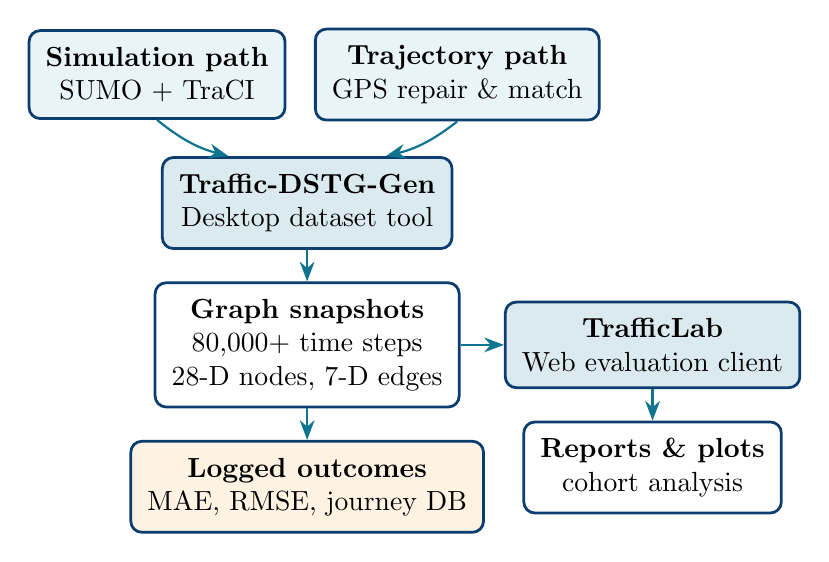
\begin{tikzpicture}[
      font=\normalsize,
      box/.style={
        draw=PosterBlue, rounded corners=4pt, align=center,
        inner sep=6pt, minimum width=3.1cm, line width=1pt,
        fill=white
      },
      arr/.style={-{Stealth[length=2.5mm]}, thick, color=PosterTeal}
    ]
      \node[box, fill=PosterLight] (sumo) {\textbf{Simulation path}\\SUMO + TraCI};
      \node[box, fill=PosterLight, right=0.35cm of sumo] (traj) {\textbf{Trajectory path}\\GPS repair \& match};
      \coordinate (m) at ($(sumo.south)!0.5!(traj.south)$);
      \node[box, below=0.45cm of m, fill=PosterTeal!15] (desk) {\textbf{Traffic-DSTG-Gen}\\Desktop dataset tool};
      \node[box, below=0.4cm of desk] (snap) {\textbf{Graph snapshots}\\80{,}000+ time steps\\28-D nodes, 7-D edges};
      \node[box, below=0.4cm of desk, right=0.55cm of snap, fill=PosterTeal!15] (web) {\textbf{TrafficLab}\\Web evaluation client};
      \node[box, below=0.4cm of snap, fill=PosterAccent!12] (out) {\textbf{Logged outcomes}\\MAE, RMSE, journey DB};
      \node[box, below=0.4cm of web] (out2) {\textbf{Reports \& plots}\\cohort analysis};
      \draw[arr] (sumo.south) to[bend right=12] ([xshift=-1cm]desk.north);
      \draw[arr] (traj.south) to[bend left=12] ([xshift=1cm]desk.north);
      \draw[arr] (desk) -- (snap);
      \draw[arr] (snap) -- (web);
      \draw[arr] (snap) -- (out);
      \draw[arr] (web) -- (out2);
    \end{tikzpicture}%
    }
    \vspace{0.5em}
    {\small Both construction paths export the \textbf{same graph schema}, enabling one training pipeline and one evaluation client.}
  }

  \column{0.32}

  \block{\Large Platform at a Glance}{
    \begin{minipage}[t]{0.48\linewidth}
      \textbf{\color{PosterTeal}Traffic-DSTG-Gen}
      \begin{itemize}
        \item Route-aware dynamic graphs from SUMO
        \item Hybrid static/dynamic nodes \& edges
        \item Simulation \& trajectory conversion
        \item Configurable temporal snapshots
        \item PySide6 desktop GUI
      \end{itemize}
    \end{minipage}\hfill
    \begin{minipage}[t]{0.48\linewidth}
      \textbf{\color{PosterTeal}TrafficLab}
      \begin{itemize}
        \item Real-time ETA inference
        \item Interactive trip evaluation
        \item Vue.js + FastAPI + PostgreSQL
        \item MAE / RMSE benchmarking
        \item Path-independent validation
      \end{itemize}
    \end{minipage}
    \vspace{0.6em}
    \begin{center}
    \begin{tabular}{@{}l r@{}}
      \toprule
      \textbf{Dataset scale} & 80{,}000+ snapshots \\
      \textbf{Node features} & 28 dimensions \\
      \textbf{Edge features} & 7 dimensions \\
      \textbf{Example bundles} & 3-zone city + Porto taxi \\
      \bottomrule
    \end{tabular}
    \end{center}
  }

\end{columns}

% ============================================================
%  Row 2 — Graph model | Desktop UI | Web UI
% ============================================================
\begin{columns}
  \column{0.34}

  \block{\Large Route-Aware Dynamic Graph}{
    \centering
    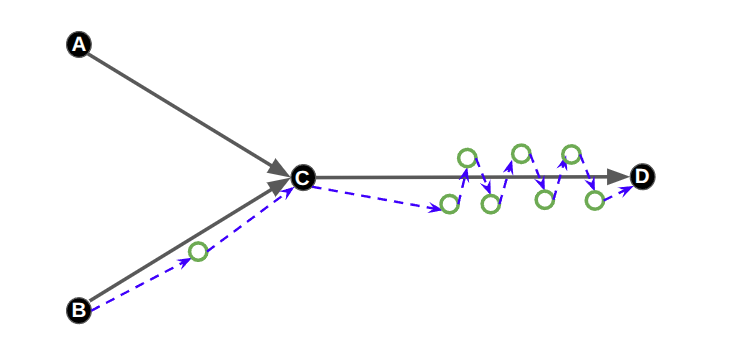
\includegraphics[width=0.92\linewidth]{../nodes.png}
    \vspace{0.4em}

    {\small
    \textbf{Static layer:} junction nodes (A--D) connected by road edges.\\
    \textbf{Dynamic layer:} vehicle nodes with dashed relations to junctions and other vehicles, updated each snapshot.\\
    \textbf{Features:} speed, position, route progress, destination --- enabling vehicle-level ETA prediction.
    }
  }

  \column{0.32}

  \block{\Large Dataset Generation (Desktop)}{
    \centering
    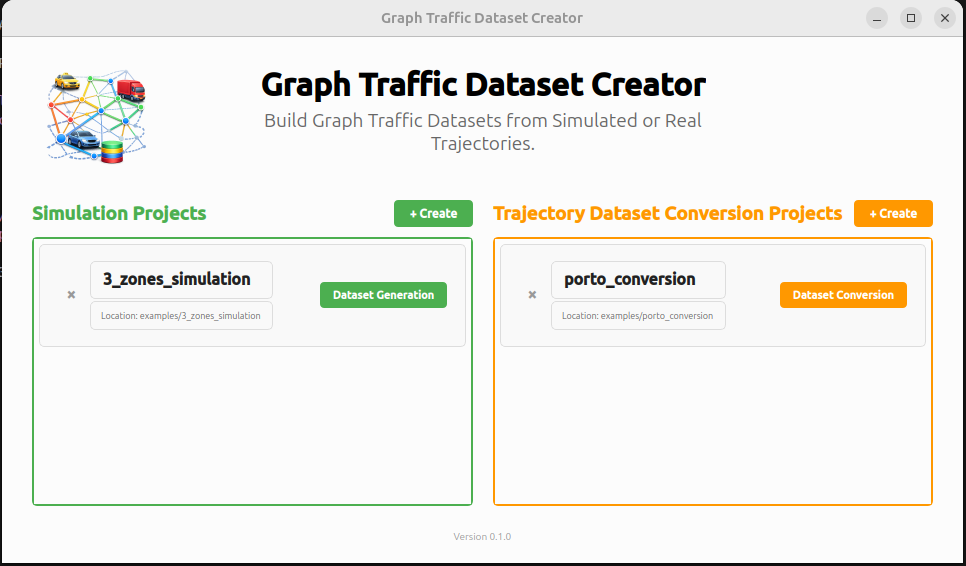
\includegraphics[width=\linewidth]{../../Academia/images/dataset_projects.png}
    \vspace{0.4em}
    {\small
    Two bundled examples: \textbf{3-zone city simulation} (left) and \textbf{Porto taxi conversion} (right). Operators configure SUMO scenarios or import GPS CSVs, validate routes on the map, and export time-stamped graph bundles for training.
    }
  }

  \column{0.34}

  \block{\Large Interactive Evaluation (Web)}{
    \centering
    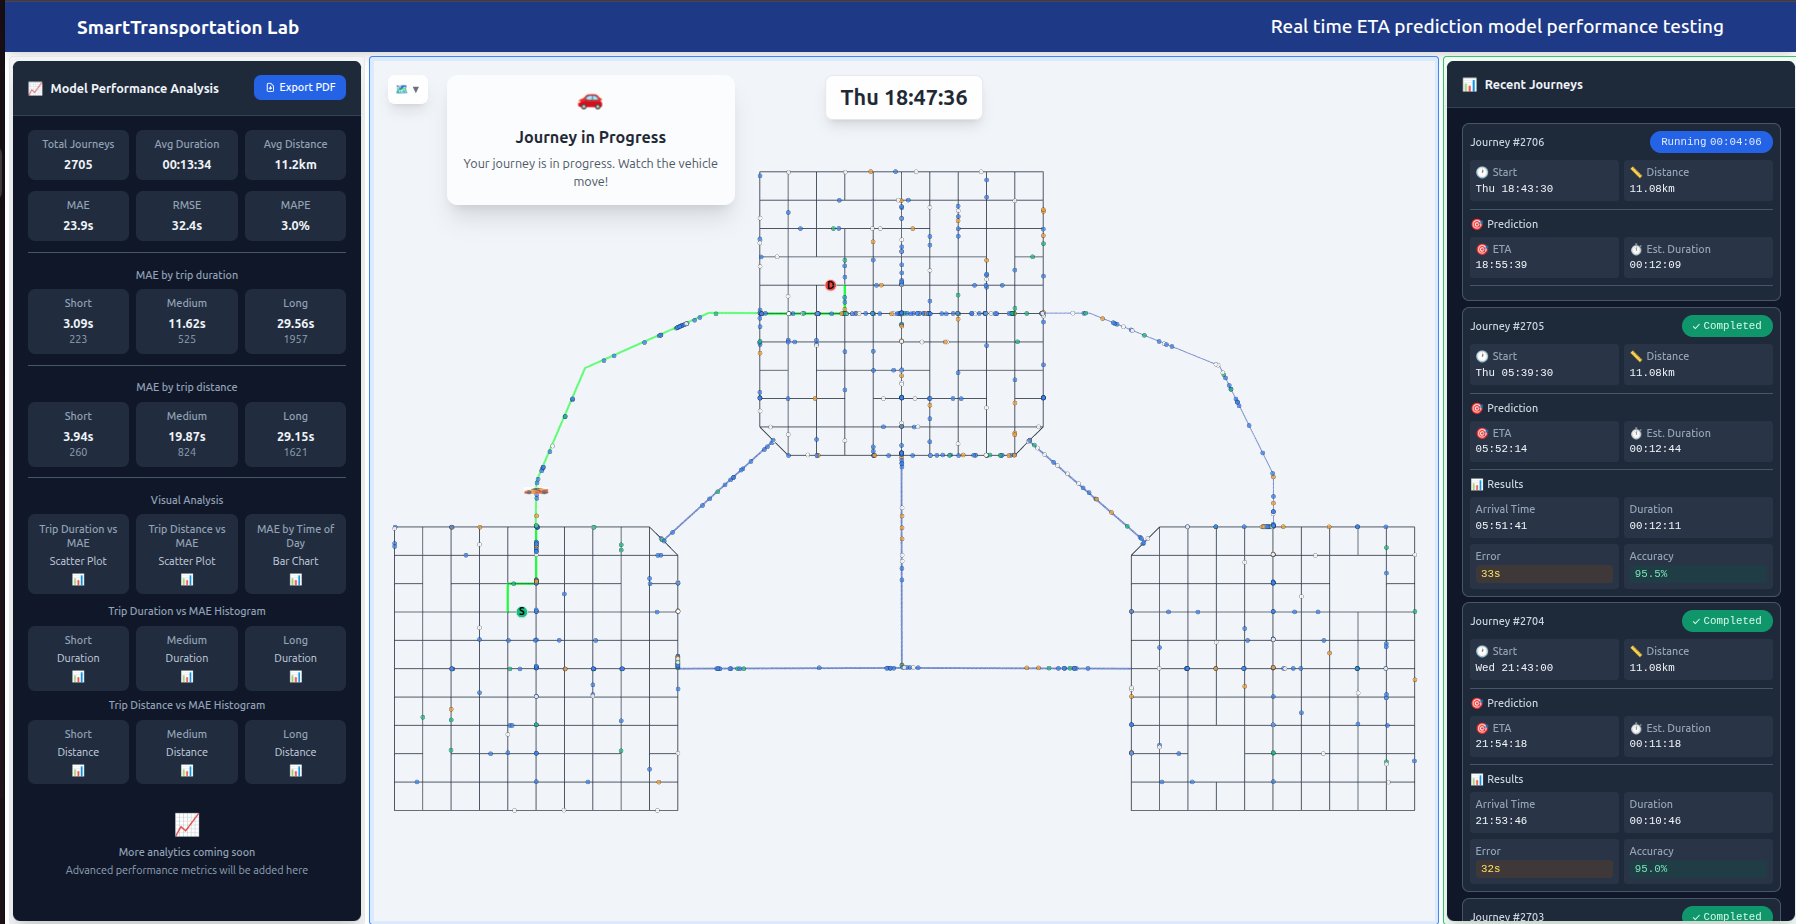
\includegraphics[width=\linewidth]{../../Academia/images/web_sim.png}
    \vspace{0.4em}
    {\small
    Users select origin/destination, receive a \textbf{predicted ETA}, run the journey in SUMO, and log realized duration. Dashboard panels show recent journeys and aggregate model performance --- the same UI works for simulation-derived and trajectory-converted networks.
    }
  }

\end{columns}

% ============================================================
%  Row 3 — Results | Example journey | Takeaways
% ============================================================
\begin{columns}
  \column{0.38}

  \block{\Large Evaluation Results}{
    \begin{minipage}[t]{0.52\linewidth}
      \centering
      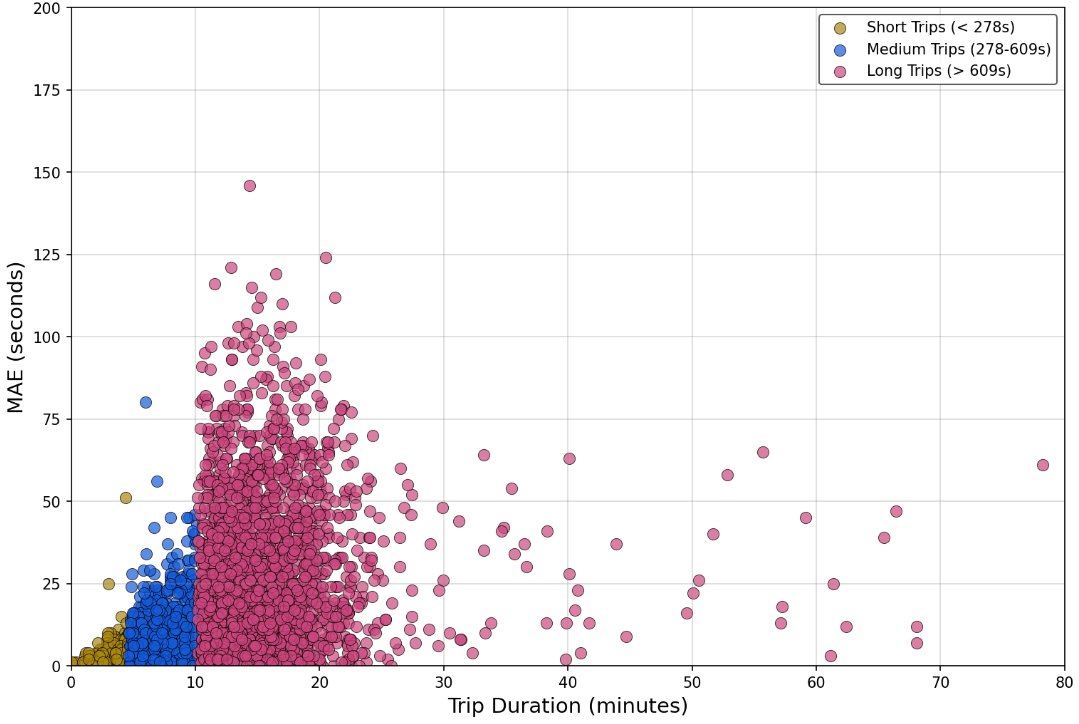
\includegraphics[width=\linewidth]{../mae_vs_time_plot_inverted.png}
      \vspace{0.3em}
      {\small MAE vs.\ trip duration (ICSEE paper figure). Short trips show lower error; the platform supports cohort analysis across duration buckets.}
    \end{minipage}\hfill
    \begin{minipage}[t]{0.44\linewidth}
      \centering
      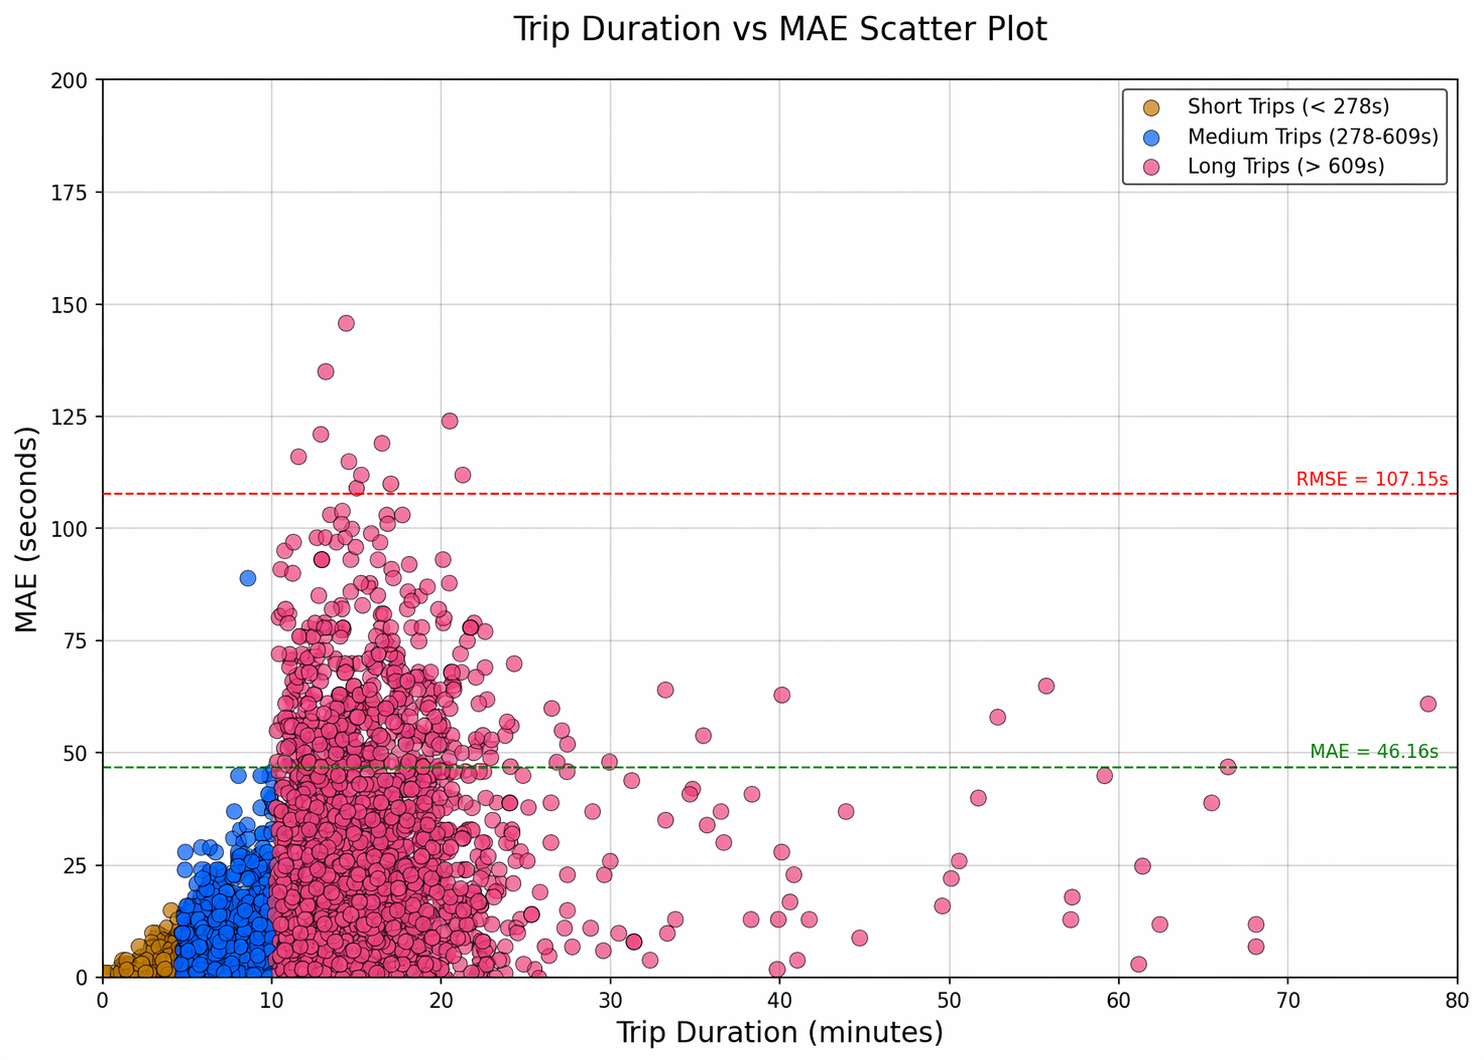
\includegraphics[width=\linewidth]{../../Academia/images/3onesmae.png}
      \vspace{0.3em}
      {\small Per-journey absolute error vs.\ duration on the simulation bundle (2{,}707 logged trips).}
      \vspace{0.8em}

      \scriptsize
      \begin{tabular}{@{}l rr@{}}
        \toprule
        & \textbf{Sim.} & \textbf{Porto} \\
        \midrule
        Journeys ($n$) & 2{,}707 & 3{,}055 \\
        MAE (s) & 46.2 & 52.4 \\
        RMSE (s) & 107.2 & 121.5 \\
        MedAE (s) & 31.2 & 35.5 \\
        \bottomrule
      \end{tabular}
      \vspace{0.4em}

      {\small Web-tool metrics closely match held-out training evaluation, confirming end-to-end integration.}
    \end{minipage}
  }

  \column{0.30}

  \block{\Large Example Journey}{
    \centering
    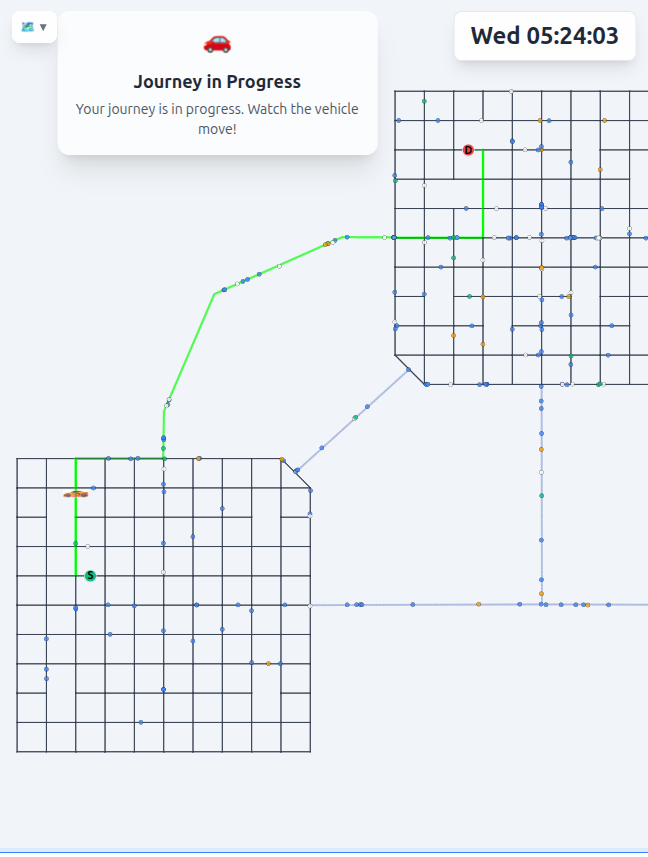
\includegraphics[width=0.88\linewidth]{../../Academia/images/web3.png}
    \vspace{0.4em}
    {\small
    Journey \#2709: 13.5\,km route, predicted duration 17:11, realized arrival within \textbf{19 seconds} (98.1\% accuracy). Each completed trip is persisted for aggregate reporting.
    }
  }

  \column{0.32}

  \block{\Large Conclusions \& Links}{
    \textbf{Contributions}
    \begin{itemize}
      \item Unified toolchain: SUMO simulation \emph{and} GPS trajectory $\rightarrow$ dynamic graphs
      \item Route-aware representation suited to vehicle-level ETA GNNs
      \item Closed validation loop from dataset export to interactive web testing
      \item Open-source release for reproducible smart-transportation research
    \end{itemize}
    \vspace{0.4em}
    \textbf{Future work:} federated learning, additional real-world data sources, broader city deployments.

    \vspace{0.6em}
    \begin{minipage}[c]{0.28\linewidth}
      \centering
      \qrcode[height=2.6cm]{https://github.com/Ruppin-SmartTransportation/Traffic-DSTG-Gen}\\[0.2em]
      {\scriptsize DSTG-Gen}
    \end{minipage}\hfill
    \begin{minipage}[c]{0.28\linewidth}
      \centering
      \qrcode[height=2.6cm]{https://github.com/Ruppin-SmartTransportation/TrafficLab}\\[0.2em]
      {\scriptsize TrafficLab}
    \end{minipage}\hfill
    \begin{minipage}[c]{0.28\linewidth}
      \centering
      \qrcode[height=2.6cm]{https://demo.smart-transport.cloud/}\\[0.2em]
      {\scriptsize Live demo}
    \end{minipage}

    \vspace{0.6em}
    {\small
    \textbf{Acknowledgment:} Supported by Ruppin Academic Center and the Israeli Ministry of Innovation, Science and Technology (Proposal 0007846); grant 34836.
    }
  }

\end{columns}

\end{document}
